{\label{exer:04_04_ex_35} The length $l$ of a long wall is to be approximated. The angle $\theta$, as shown in the diagram (not to scale), is measured to be $85.2^\circ$, accurate to $1^\circ$. Assume that the triangle formed is a right triangle.

\begin{minipage}{\linewidth}
\centering
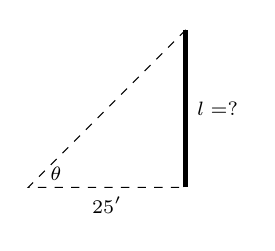
\begin{tikzpicture}
\draw [ultra thick] (1,-1) -- node [pos=.5,right] {\scriptsize $l=$?}(1,1);
\draw [dashed] (1,1) -- (-1,-1) node [xshift=10pt,yshift=5pt] {\scriptsize $\theta$} -- node [pos=.5,below] {\scriptsize $25'$} (1,-1);
%\draw (-.5,0) -- node [pos=.5,draw=white,fill=white] {\scriptsize $50'$} (1,0);
\end{tikzpicture}
\end{minipage}

\begin{enumerate}
\item		What is the measured length $l$ of the wall?
\item		What is the propagated error? 
\item		What is the percent error?
\end{enumerate}
}
{\begin{enumerate}
\item		297.8 feet
\item		$\pm 62.3$ ft
\item		$\pm 20.9$\% 
\end{enumerate}
}

